\customHeader{1}{\neuralNetwork{}s}
\label{02_neural_networks}




In this section, we present the fundamental concepts necessary for understanding \neuralNetwork{}s, drawing on the Open Access material from \mytextcite{deep_learning_introduction} and \mytextcite{wolfram_llm}.

\customHeader{2}{Motivating Example}
\label{02_nn_motivating_example}


To understand the rationale behind using \neuralNetwork{}s, let's consider a scenario where we aim to determine how the temperature and humidity of a place relate to the perceived temperature by living beings, such as humans. In other words, given these two metrics across various locations, our goal is to forecast the felt temperature or Heat Index for each site. A simplified version of the model from \mytextcite{heat_index}, can provide us with an equation for the Heat Index ($HI$).

\begin{align*}
    HI &= w_{Temp} T + w_{Hum} H + c
\end{align*}


The main idea behind this model is that the heat index, our \emph{target}, can be calculated as a weighted sum of the temperature $T$ and the humidity $H$. The influence of $T$ on the $HI$ is given by $w_{Temp}$ and that of $H$ by $w_{Hum}$, and we correct by a constant value $c$. 

In this model, $H$ and $T$ are termed the \emph{features} of a location, serving as its defining characteristics. Essentially, locations with identical features will yield the same output. The terms $w_{Temp}$ and $w_{Hum}$ are referred to as \emph{weights} or \emph{parameters}. They signify the relevance of the features to the model. For instance, if $w_{Hum}$ is zero, the $HI$ would solely be influenced by $T$. Additionally, $c$ is labeled as the \emph{bias} or \emph{offset}, representing the output value when the features are null. The equation's right-hand side, $w_{Temp} T + w_{Hum} H + c$, is recognized as the model's \emph{output} or \emph{prediction}.


In practice, the values for the weights and bias of this model have been determined to be:
\begin{align*}
w_{Temp} & = 1.1\\
w_{Hum} &= 0.047 F^\circ \\
c &= -10.3 F^\circ
\end{align*}

Yet, this basic representation has its limitations. Interestingly, by introducing an additional computational step, we can achieve more accurate results. Let's consider incorporating a minor squared term through the function $f(u) = u + 0.0002 u^2$. With this, our model evolves to:

\begin{align*}
HI &= f(w_{Temp} T + w_{Hum} H + c)
\end{align*}

In this enhanced model, $f$ is termed the \emph{activation function}. The model's prediction or output is derived by applying $f$ to the weighted sum. This added computation step allows for a more authentic representation of how living beings respond to significant shifts in temperature and humidity. 
In general, this kind of model allows us to use numerical features, to obtain a prediction for a variable of interest.

\customHeader{2}{Neurons}
\label{02_nn_neurons}




When dealing with increasingly complex phenomena, it becomes challenging to explicitly define the parameters for a model. This requires a broader approach. In the realm of Machine Learning, the concept of \emph{neurons} serves as a generalization of the model described earlier.




\begin{figure}[ht]
    \centering
    \subfigure[Neuron overview]{
    \begin{tikzpicture}[scale=0.7, every node/.style={transform shape}]
        % Add the "Hello" text to the left
        \node[anchor=east] at (-3, 0) {Input};
        
        % Draw the neuron circle with a node name
        \node[draw, thick, circle, minimum size=1.5cm, fill=mylightblue] (neuron) at (0, 0) {};
        
        % Draw the input nodes with labels x_i
        \foreach \x/\xval in {1/{$x_1$}, 2/{$x_2$}, 3/{$x_3$}} {
            \node[draw, circle, minimum size=0.7cm] (input\x) at (-2, 2.8-\x*1.4) {};
            \draw[->] (input\x) -- node[above] {} (neuron);
        }
        
        % Draw the output arrow
        \draw[->] (neuron) -- (2, 0) node[right] {Output};
    \end{tikzpicture}
    }
    \hfill
    \subfigure[Neuron with weights]{
    \begin{tikzpicture}[scale=0.7, every node/.style={transform shape}]
        % Add the "Hello" text to the left
        \node[anchor=east] at (-3, 0) {Input};
        
        % Draw the neuron circle with a node name
        \node[draw, thick, circle, minimum size=1.5cm, fill=mylightblue] (neuron) at (0, 0) {$f$};
        
        % Draw the input nodes with labels x_i
        \foreach \x/\xval in {1/{$x_1$}, 2/{$x_2$}, 3/{$x_3$}} {
            \node[draw, circle, minimum size=0.7cm] (input\x) at (-2, 2.8-\x*1.4) {\xval};
            \draw[->] (input\x) -- node[above] {$w_\x$} (neuron);
        }
        
        % Draw the output arrow
        \draw[->] (neuron) -- (2, 0) node[right] {$z$ Output};
    \end{tikzpicture}
    }
    \caption{
    Basic Neuron
    }
    \label{fig:02_neuron}
\end{figure}


Consider a model where the inputs encompass $n$ distinct features, represented as $(x_1, x_2,\ldots,x_n)$. The diagram depicted in Figure \ref{fig:02_neuron} represents the following equation:

\begin{align*}
z &= f(w_1 x_1 + w_2 x_2 + \ldots + w_d x_d + b)
\end{align*}

Here, $w_1, w_2,\ldots,w_n$ denote the weights, $b$ signifies the bias, $f$ is the activation function, and $z$ stands for the prediction.

One of the main insights in \gls{ml} is that one does not need to manually define the parameters $(w_1, w_2,\ldots,w_n,b)$ for this kind of model.
Instead, with ample data comprising input features and observed target values, it is feasible to determine the best parameter values. This ensures the model's predictions closely align with the observed target values. Once established, this model can be applied to new data. The process of finding the optimal parameters is called \emph{training}.

In order to find the optimal parameters, we first need to decide how to produce our final predictions, how to measure how well the model is performing, and how to update the model's parameters.


\customHeader{2}{Activation functions}
\label{02_nn_activation_functions}


The method used to derive our final predictions is contingent on the specific problem to be addressed. Various activation functions cater to different problems. For instance, in \emph{regression}, where our objective is to compute a continuous quantity,  like in the example in \headerName{} \ref{02_nn_motivating_example}, we may handle values that can range from extremely small to exceedingly large. On the other hand, classification tasks aim to predict a categorical label, either by taking a final decision or by producing probabilities for each category.


Table \ref{tab:02_nn_common_activation_functions} and Figure \ref{fig:02_nn_common_activation_functions} enumerate some of the most common activation functions.

\begin{table}%[]
    \centering
    \begin{tabular}{p{4cm}|p{8cm}}
        \textbf{Activation Function} &  \textbf{Description} \\ \hline
        Identity &  No modification to the weighted sum\\
        \gls{relu} & Eliminates negative values. Better for optimization \\
        \gls{sigmoid} & Outputs a single probability \\
        \gls{softmax} & Generalization of \gls{sigmoid} for multiple categories. Outputs a list of probabilities. \\
        \gls{tanh} & Reduces the influence of huge and minuscule values. Better for optimization \\
    \end{tabular}
    \caption{Common activation functions}
    \label{tab:02_nn_common_activation_functions}
\end{table}


\begin{figure}[ht]
    \centering
    \subfigure[Identity]{
        \begin{adjustbox}{max height=0.07\textheight}
            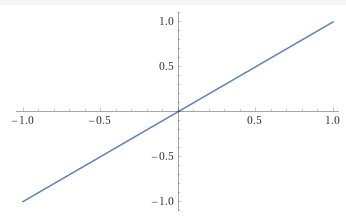
\includegraphics[width=0.45\textwidth]{Figures/02/Activation_functions/02_Identity.png}
        \end{adjustbox}
        
        %\label{fig:image1}
    }
    \hfill
    \subfigure[ReLU]{
        \begin{adjustbox}{max height=0.07\textheight}
            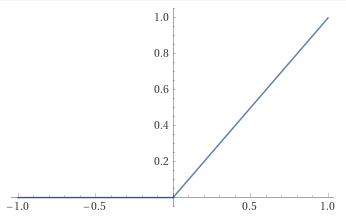
\includegraphics[width=0.45\textwidth]{Figures/02/Activation_functions/02_Relu.png}
        \end{adjustbox}
        
        %\label{fig:image2}
    }
    \hfill
    \subfigure[Sigmoid]{
        \begin{adjustbox}{max height=0.07\textheight}
            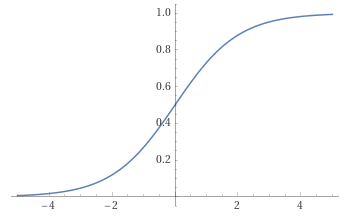
\includegraphics[width=0.45\textwidth]{Figures/02/Activation_functions/02_sigmoid.png}
        \end{adjustbox}
        
        %\label{fig:image1}
    }
    \hfill
    \subfigure[Tanh]{
        \begin{adjustbox}{max height=0.07\textheight}
            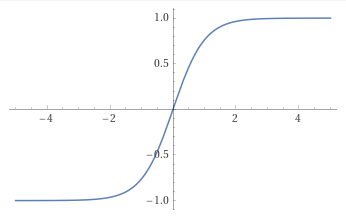
\includegraphics[width=0.45\textwidth]{Figures/02/Activation_functions/02_tanh.png}
        \end{adjustbox}
        
        %\label{fig:image2}
    }
    \caption{Common activation functions}
    \label{fig:02_nn_common_activation_functions}
\end{figure}





\customHeader{2}{Loss Functions}
\label{02_nn_loss_functions}


Loss functions quantify the deviation of predicted values from actual target values. The goal during training is to adjust the parameters to minimize this deviation. The process of inputting data into the neuron to compute the loss is termed the \emph{forward pass}.

For regression tasks, the squared error is frequently employed. It calculates the squared difference between the predicted and actual values:

\begin{equation}
loss_{SE}(x,w,b) = \dfrac{1}{2} (z_{pred}(x,w,b)-z_{real})^2
\end{equation}

where $z_{pred} = f(xw+b)$.

In classification tasks, the \emph{cross-entropy} loss is common. The essence of cross-entropy is to maximize the model's confidence in its category assignments\footnote{Deducing the formula for Cross-Entropy is outside the scope of this work}. Given features $x = x_1, x_2, \ldots, x_n$ and predicted probabilities $p_1, p_2, \ldots, p_k$ for categories $c_1, c_2, \ldots, c_k$, and representing actual categories as $(q_1, q_2, \ldots, q_k)$ where $q_j =1 $ for category $j$ and $q_j = 0$ otherwise, cross entropy is:

\begin{equation}
loss_{CE}(x,w,b) = - \sum_{j} q_{j}(x) \log{(p_{j}(x,w,b))}
\end{equation}

For datasets with uneven category distribution, or \emph{unbalanced} datasets, a modified version called \emph{weighted cross-entropy} can be used. It adjusts the cross-entropy based on category representation. If category $j$ has a weight of $r_j$, then:

\begin{equation}
loss_{WCE}(x,w,b) = - \sum_{j} r_j q_{j}(x) \log{(p_{j}(x,w,b))}
\end{equation}


\customHeader{2}{Backpropagation}
\label{02_nn_loss_back_propagation}

After measuring the performance of a neuron through the loss, our aim is to adjust its parameters to reduce this loss. The process of \emph{updating} the weights to achieve this reduction is termed \emph{backpropagation}. A common  optimization technique to achieve this is \emph{gradient descent}. For illustrative purposes, let's assume that the neuron has just one weight, and thus, there's just one weight influencing the loss (as depicted in Figure \ref{fig:02_nn_gradient_descent}). The key insight is that moving against the slope of the loss curve brings us closer to its minimum. This slope is the derivative or the \emph{gradient} of the loss function. Through several iterative steps, updating the weight each time, we eventually reach the ideal weight that minimizes the loss.

\begin{figure}
\centering
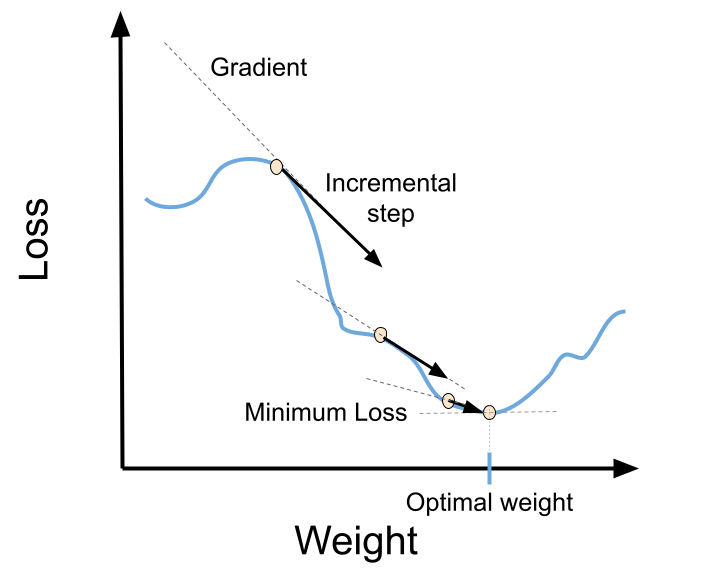
\includegraphics[width=0.5\textwidth]{Figures/02/02_gradient_descent.png}
\caption{Gradient descent illustration}
\label{fig:02_nn_gradient_descent}
\end{figure}

Having identified the direction of adjustment, it's also crucial to regulate the magnitude of this adjustment. This is achieved using the \emph{learning rate} $\eta$, which moderates the gradient's impact on weight updates. That is, our weight updating process is calculated in the following way:

\begin{align}
w_{new} = w_{old} - \eta \nabla loss(x, w_{old}) \label{eq:02_nn_gradient_descent}
\end{align}



% gradient descent
% learning rate
% loss optimization

\customHeader{2}{Training}
\label{02_nn_training}



Up to this point, we've discussed using just one feature vector as input for a neuron. But for a comprehensive representation of our task, multiple examples are essential. This means, for effective training, we require multiple data points, or in other words, a \emph{Dataset} comprising both features and their corresponding observed target values $(x,z_{real})$. If our Dataset $D$ contains $N$ items, our goal becomes minimizing the \emph{average} loss across the dataset:

\begin{equation}
Loss(w,b) = \dfrac{1}{N} \sum_{x\in D} loss(x,w,b)
\end{equation}

The entire process of executing the forward pass, determining the loss, and updating weights through backpropagation is termed an \emph{epoch} (as illustrated in Figure \ref{fig:02_nn_neuron_training}).

\begin{figure}
\centering
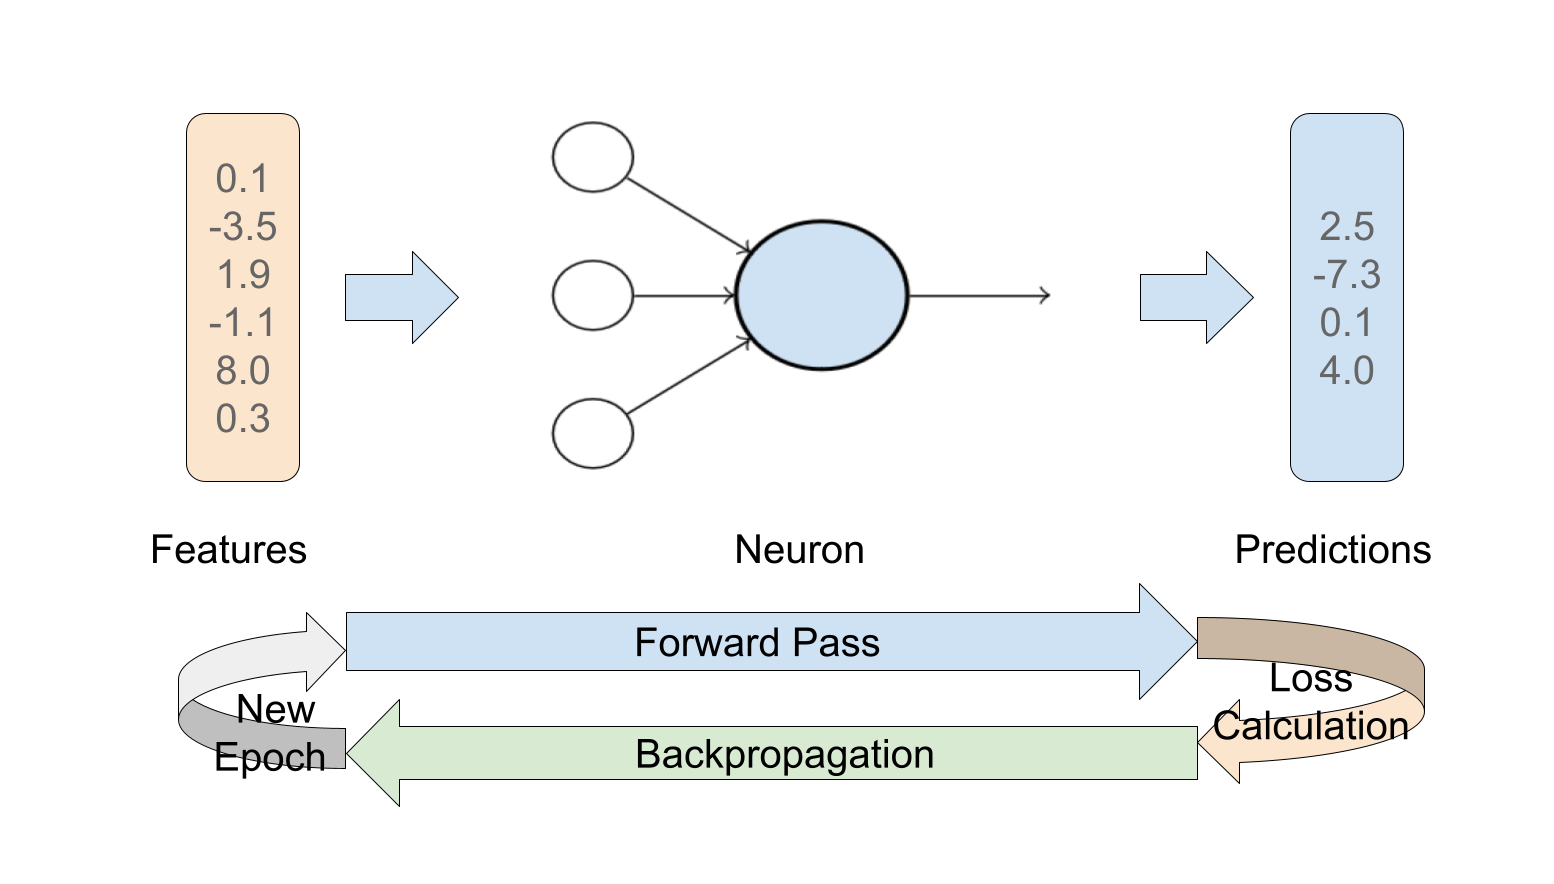
\includegraphics[width=0.75\textwidth]{Figures/02/02_neuron_training.png}
\caption{Neuron Training Process}
\label{fig:02_nn_neuron_training}
\end{figure}

In most cases, our computing resources might not possess the capacity to process the entire Dataset in one run. A common workaround is segmenting the Dataset into equally sized \emph{batches}. The forward pass and loss computation are then executed batch by batch until the entire dataset is covered. Subsequently, the losses from each batch are combined to determine the final loss, followed by backpropagation. Typical batch sizes include powers of 2: $2, 4, 8, 16, 32, 64, \ldots, 2^n, \ldots$

Often, a single epoch doesn't suffice to yield satisfactory outcomes. Hence, it's a standard practice to train a neuron over multiple epochs. With each epoch, the loss typically reduces (as depicted in Figure \ref{fig:02_nn_loss_evolution}).

\begin{figure}
    \centering
    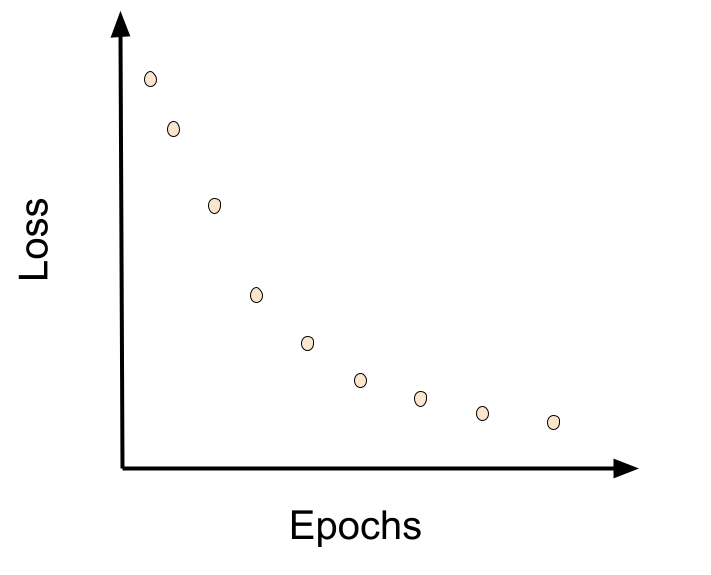
\includegraphics[width=0.5\textwidth]{Figures/02/02_loss_evolution.png}
    \caption{Evolution of loss during training}
    \label{fig:02_nn_loss_evolution}
\end{figure}

% batches
% epochs

\customHeader{2}{Overfitting }
\label{02_nn_overfitting}


As we progressively reduce our loss, we encounter a challenge. There are instances when the neuron will produce excellent predictions for the data it was trained on, but performs poorly on entirely new data, rendering the neuron useless for real-world applications. This issue is termed \emph{overfitting}.

A prevalent strategy to counteract overfitting is to \emph{divide} the dataset into three distinct portions:

\begin{enumerate}
\item The \emph{training} split, which constitutes a portion of the dataset dedicated to the core training processes, including the forward pass, loss evaluation, and crucially, backpropagation.
\item The \emph{development} split, a portion of the dataset designated for tracking potential overfitting. For this split, we execute the forward pass and compute the loss, and occasionally other metrics, but refrain from backpropagation. Recognizing the beginning of overfitting allows us to adjust our setup for the optimal number of epochs.
\item The \emph{test} split, a portion of the dataset reserved for assessing the efficacy of the chosen training setup, especially since this subset wasn't involved in its selection.
\end{enumerate}

When monitoring the trajectory of the loss across the training and development splits, a pattern emerges. After a specific number of epochs, the loss on the training split continues to drop, but the development split's loss starts to climb. This shift marks the beginning of overfitting (depicted in Figure \ref{fig:02_nn_split_loss_evolution}).

\begin{figure}
    \centering
    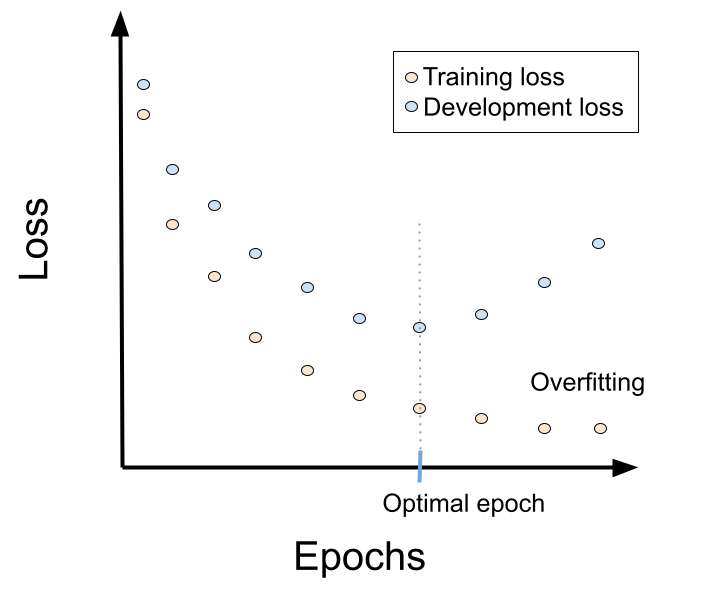
\includegraphics[width=0.5\textwidth]{Figures/02/02_split_loss_evolution.png}
    \caption{Evolution of loss on the training and development splits}
    \label{fig:02_nn_split_loss_evolution}
\end{figure}


% splits.
% plot for optimal epoch

\customHeader{2}{Optimizers }
\label{02_nn_optimizers}

% optimizers
We may generalize Gradient Descent (Equation \ref{eq:02_nn_gradient_descent}), by noticing that we only need to calculate some way to update our weights:

\begin{equation}
    w_{new} = w_{old} - \texttt{Update}(x, w_{old})
\end{equation}

Different optimization methods calculate the \texttt{Update} in different ways. Software implementations of these optimization methods are called \emph{optimizers}. Some common methods are listed in Table \ref{tab:02_nn_common_optimizers}, listed by increasing performance.

\begin{table}%[]
    \centering
    %\resizebox{0.75\textwidth}{!}{
    \begin{tabular}{p{0.3\textwidth}|p{0.6\textwidth}}
        \textbf{Optimization method} &  \multicolumn{1}{c}{\textbf{Description}} \\ \hline
        Gradient Descent &  Classical Gradient Descent\\
        Stochastic Gradient Descent (SGD) & Estimates the gradient by only using a randomly selected subset of the data \\
        SGD with Momentum & Uses the estimated gradient and the previous value of \texttt{Update}\\
        Averaged SGD &  Takes into account several past values of \texttt{Update} and averages them while giving less importance to older values \\
        Adaptive Gradient (AdaGrad) & A version of SGD where each weight is updated with its own learning rate, instead of all weights using the same one. It calculates \texttt{Update} by averaging and normalizing over the history of updates \\
        Adam & AdaGrad + Momentum \\
        AdamW & Extension of Adam, controlling for the magnitude of each weight \\
    \end{tabular}
    %}
    \caption{Common optimization methods for backpropagation}
    \label{tab:02_nn_common_optimizers}
\end{table}



\customHeader{2}{Feed-Forward \neuralNetwork{}s}
\label{02_nn_ffnn}

As we have seen, an individual neuron may take several inputs to give an output, and this provides us with a model useful for some applications. 
One of the groundbreaking insights in \gls{ml} was the idea of linking neurons together. This involves using the output of one neuron as the input for others. By organizing neurons into \emph{linear layers} and interconnecting them, we create a \gls{ffnn} (Refer to Figure \ref{fig:02_nn_ffnn})\footnote{All diagrams of \neuralNetwork{} were made with the $NN-SVG$ tool by \mytextcite{drawing_nns}}.

\begin{figure}
    \centering
    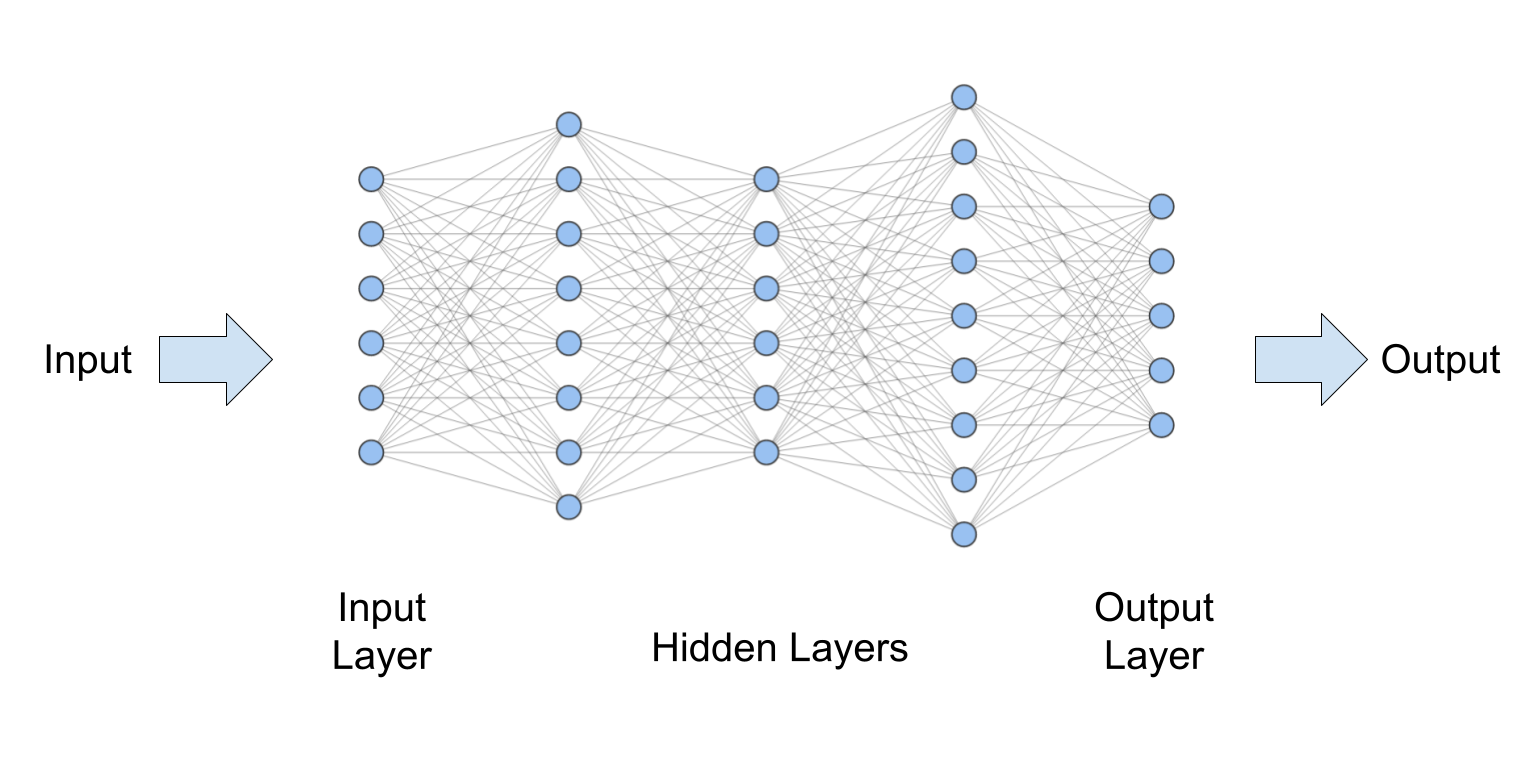
\includegraphics[width=0.75\textwidth]{Figures/02/02_FFNN.png}
    \caption{A Feed-Forward \neuralNetwork{}}
    \label{fig:02_nn_ffnn}
\end{figure}

When performing the forward pass, input features are fed into the \gls{ffnn} via the \emph{input layer}, they traverse through intermediate layers until they reach the \emph{output layer}.
As the \gls{ffnn} undergoes training, every intermediate layer crafts new features for the subsequent layers. 
This mechanism enables the \gls{ffnn} to \emph{learn} new representations for the data.
These in-between, or \emph{hidden}, features detect and leverage patterns from earlier features to determine the final output of the \neuralNetwork{}. A \neuralNetwork{} with just one hidden layer is termed \emph{shallow}, whereas those with several hidden layers are called \emph{deep}.

For classification tasks, the \gls{softmax} activation function is typically employed in the output layer since it yields a probability distribution across various categories. Such a layer is termed a \emph{\gls{softmax} layer} or a \emph{classification layer}. The inputs to this layer are often referred to as \emph{logits}. Given that we're working with probabilities, the objective is to minimize the cross-entropy loss between the predictions of the \neuralNetwork{} and the true labels.
(Refer to Figure \ref{fig:02_nn_nns_for_classification})

\begin{figure}
    \centering
    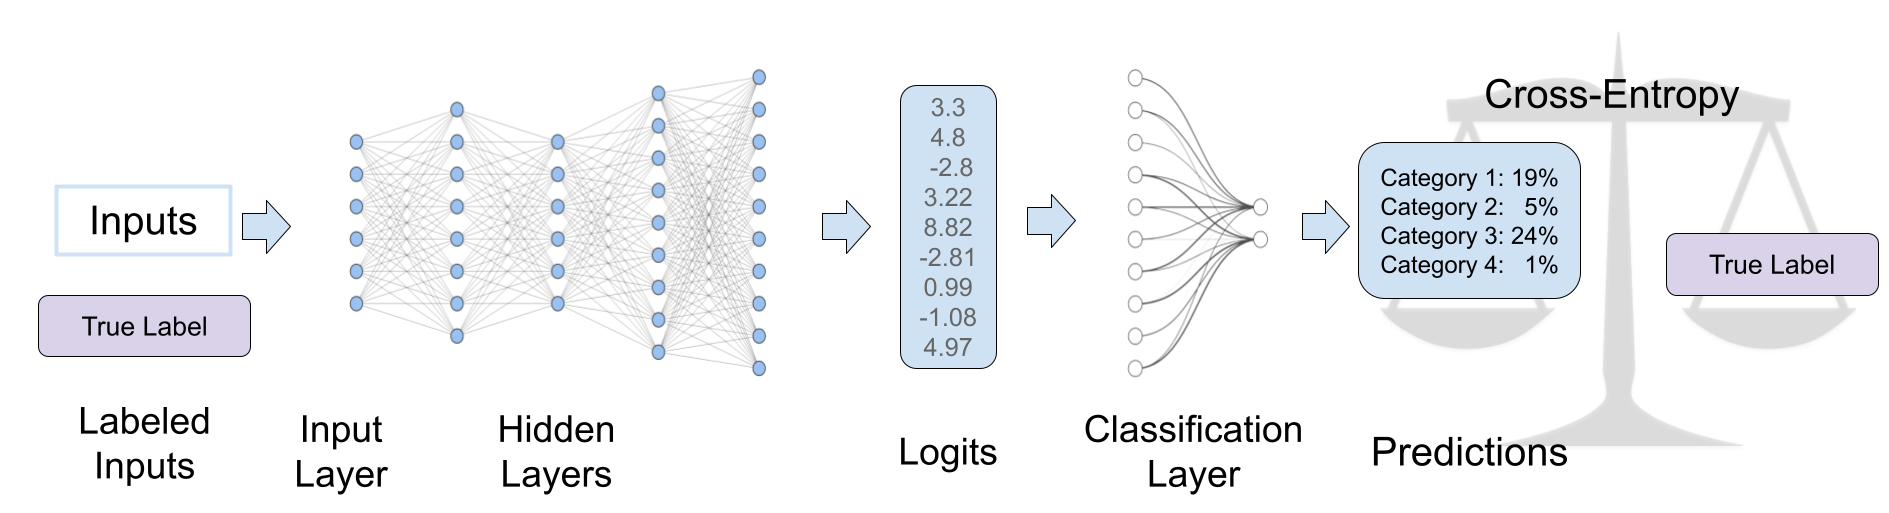
\includegraphics[width=\textwidth]{Figures/02/02_nns_for_classification.png}
    \caption{\neuralNetwork{}s for Classification Tasks}
    \label{fig:02_nn_nns_for_classification}
\end{figure}


% FF NN
% deep vs shallow
% softmax layers
% diagram with the full training cycle

\customHeader{2}{Hyperparameters}
\label{02_nn_hyperparameters}

When training a \neuralNetwork{}, the goal is to progressively adapt its parameters or weights to minimize the loss. However, several critical choices need to be made by the designers of the \neuralNetwork{}.

Some decisions concern the \emph{architecture} of the \neuralNetwork{}, such as:

\begin{itemize}
    \item Number of layers
    \item Number of Neurons per layer
    \item Activation functions for each layer
    \item Dimension of output features
    \item Loss function
    \item Optimizer
\end{itemize}

There are also decisions about specific numerical values that affect the training method, such as:


\begin{itemize}
    \item Number of epochs
    \item Learning rate
    \item Batch size
    \item Sizes for the dataset splits
\end{itemize}

All these are known as \emph{hyperparameters}. Unfortunately, there is no one-size-fits-all answer to the question of which hyperparameters to use because the optimal hyperparameters can vary depending on the specific dataset, model architecture, and task at hand. The search space for hyperparameters can be vast, and finding the best combination can be computationally expensive and time-consuming. As a result, the choice of hyperparameters is often determined through trial and error, experimentation, and a combination of domain knowledge and experience.

%% Hyperparameters
% learning rate
% epochs
% batch size
% training, dev, and test split size


%% architecture
% dimension of input features
% activation functions
% number of layers
% neurons per layer

\customHeader{2}{\neuralNetwork{}s for NLP tasks}
\label{02_nn_nlp_tasks}

For \neuralNetwork{}s to handle \gls{nlp} tasks, textual data must be transformed into numerical features to feed to the network. 
A significant advancement in \gls{nlp} came when experts discovered that instead of handcrafting algorithms for feature generation, they could train \neuralNetwork{}s to produce these features for subsequent \neuralNetwork{}s.
The next section elaborates on this approach.



%\clearpage